\documentclass[a4paper]{article}
\usepackage{fullpage}
\usepackage[scaled]{helvet}

% Fix \paragraph to have a newline
\makeatletter
\renewcommand\paragraph{\@startsection{paragraph}{4}{\z@}%
  {-3.25ex\@plus -1ex \@minus -.2ex}%
  {1.5ex \@plus .2ex}%
  {\normalfont\normalsize\bfseries}}
\makeatother

\setcounter{secnumdepth}{4}	% Number \paragraphs

\renewcommand\maketitle{
%\ifpdf
\pdfinfo{
   /Author (\getauthor)
   /Title  (\getprojectname  - \gettitle)
   /Producer (John Hodge)
}
%\fi


\begin{titlepage}

\begin{center}

\vspace{1cm}

\textsc{\LARGE \getprojectname}\\[0.5cm]
\textsc{\huge \gettitle}\\[0.5cm]
\rule{0.9\textwidth}{0.7pt} \\[0.75cm]
% Authors
\emph{\getauthor} \\[0.5cm]
% Client
Client: \emph{\getclient} \\[0.5cm]

CITS3200 Professional Computing 2011 \\
University of Western Australia Crawley, WA, 6009

\vspace{2cm}
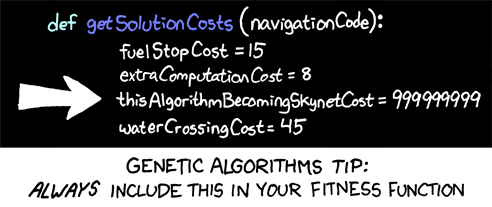
\includegraphics{../534-genetic_algorithms.png} \\
\centering{\footnotesize XKCD \#534 - Genetic Algorithms - CC BY-NC 2.5}

\end{center}

\end{titlepage}
}

\def\csharp{\ensuremath{C\sharp } }

\def\getprojectname{}
\def\projectname#1{\gdef\getprojectname{#1}}
\def\getclient{}
\def\client#1{\gdef\getclient{#1}}
\makeatletter
\newcommand\gettitle{\@title}
\newcommand\getauthor{\@author}
\makeatother

\projectname{Genetic Engine Project}
\title{Requirements Analysis Document}
\author{Rohit Gopalan, John Hodge, Alwyn Kyi, Brian Marshall, Antriksh Srivastava}
\client{Mr Peter Th\"onell}

% Set up the header
\pagestyle{fancy}
\renewcommand{\headheight}{15pt}
% Clear Old
\fancyhead{} \fancyfoot{}
% Set new
\fancyhead[C]{\small{Requirements Analysis Document}}	% Top Center (Odd/Even)
\fancyhead[R]{\small{CITS3200 Group J}}	% Top Right (Odd/Even)
\fancyfoot[R]{\thepage \slash \pageref{LastPage}}	% Bottom Right (Odd/Even)
% Line width
\renewcommand{\headrulewidth}{0.4pt} \renewcommand{\footrulewidth}{0.4pt}
% Distance from the line to the content
\renewcommand{\headsep}{24pt}

\begin{document}

\maketitle

\subsection*{Revision History}
\begin{tabularx}{\textwidth}{l c c X}
 \hline
 Version & Author & Date & Reason \\
 \hline \hline
 r1 & R. Goplan & 08/08/2011 & Created \\ \hline
 r2 & R. Goplan & 16/08/2011 & Modified 3.5 \\ \hline
 r3 & B. Marshall & 32/08/2011 & Modified 3.2 - 3.4 \\ \hline
 r4 & J Hodge & 24/08/2011 & Modified Section 2.0 \\ \hline
 r5 & R Gopalan & 24/08/2011 & Modified Section 1.0 \\ \hline
 r6 & B Marshall & 25/08/2011 & Modified Sections 3.2 to 3.4 \\ \hline
 r7 & B Marshall & 25/08/2011 & Modified Section 3.2 \\ \hline
 r8 & R Gopalan & 26/08/2011 & Modified Section 3.2 \\ \hline
 r9 & R Gopalan & 08/09/2011 & Modified Meeting Dates \\ \hline
 r10 & J Hodge & 12/09/2011 & LaTeX-ify \\ \hline
 r11 & R Gopalan & 13/09/2011 & Modified Section 3.2 \\ \hline
 r12 & B Marshall & 14/09/2011 & Added Sections 3.5.3 and 3.5.4 \\ \hline
\end{tabularx}

\subsection*{Client Sign-off}
I, Peter Thonell have read the Requirements Analysis Document and have agreed that the information provided by the Genetic Engine Project Team is accurate according to my own needs. By signing this document, I also agree that the prototypes provided by this team, are also accurate as possible to my requirements
\\[10pt]
Signed: \rule{3cm}{.7pt}
\\[10pt]
Date: \rule{0.8cm}{.7pt} \slash \rule{0.8cm}{.7pt} \slash \rule{3cm}{.7pt}

If there are any issues, with the Requirements Analysis Document and the prototypes, please attach suggestions for improvement to this document.


\subsection*{Preface}
This document addresses the requirements of the Genetic Engine system. The intended audience for this document are the designers and the client of the project.

\subsection*{Target Audience}
Client, Developers

\subsection*{CITS3200 Group J Members}
\begin{tabular}{c l}
 Group Member & Main Role \\
 \hline \hline
 Rohit Gopalan & Project Leader and User Interface Developer \\ \hline
 John Hodge & API Developer \\ \hline
 Brian Marshall & API Developer \\ \hline
 Alwyn Kyi & API/User Interface Tester \\ \hline
 Antriksh Srivastava & API/User Interface Tester\\ \hline
\end{tabular}

\subsection*{Meeting Times}
\begin{itemize}
\item Group Meeting was held on 08/08/2011, 10am at Hacket Hall Caf\'e, University of Western Australia
\item Client Meeting was held on 08/08/2011, 11am at Hacket Hall Caf\'e, University of Western Australia
\item Group Meeting was held on 15/08/2011, 1pm at Lab 2.01 in CSSE School, UWA
\item Client Meeting was held on 17/08/2011, 2pm at Reid Library, UWA
\item Group Meeting was held on 22/08/2011, 11am at Hacket Hall Caf\'e, UWA
\item Client Meeting was held on 24/08/2011, 2pm at Reid Library, UWA
\item Group Meeting was held on 29/08/2011, 11am at Hacket Hall Caf\'e, UWA
\item Client Meeting was held on 31/08/2011, 2pm at Reid Library, UWA
\item Group Meeting was held on 05/09/2011, 11am at Hacket Hall Caf\'e, UWA
\item Client Meeting was held on 07/09/2011, 2pm at Reid Library, UWA
\item Group Meeting was held on 12/09/2011, 11am at Hacket Hall Caf\'e, UWA
\item Client Meeting to be held on 14/09/2011, 2pm at Reid Library, UWA
\end{itemize}

Future Group meeting times will happen every Monday from September 19 2011 until October 17 2011. Venues to be decided later.

Future Client Meeting times will happen every Wednesday from October 5 2011 until October 19 2011. Venues to be decided later. 

\clearpage

\tableofcontents

\clearpage


%
% General Goals
%
\section{General Goals}
The aim of the system is to provide a general implementation of a genetic algorithm. 
This will be done by providing an API through the .Net library in \csharp. 
% For this section, enter the goals of your subsystem, i.e. what are the objectives of the functions of your subsystem?


%
% Current System
%
\section{Current System}
There is no current system. We are building a brand new system from scratch.
%For this section, describe the current situation that is relevant to your subsystem.


%
% Proposed System
%
\section{Proposed System}
\subsection{Overview}
The core of this system will be a .Net DLL with the implementation of the genetic engine. It will accept plug-ins to set the behaviour of various stages of the algorithm. These plug-ins will be contained in .Net DLL files and will implement interfaces defined in a support library.
A windows application will provide a graphical user interface to the genetic engine. It will allow the user to select plug-ins and set various parameters then run the algorithm.
A set of sample plug-ins are also required to solve a problem given by the client: Given a map with the locations of a number of towns and start and end points produce a network of roads which includes the start and end points and balances two goals:
\begin{enumerate}
\item Minimise the total length of the roads.
\item Minimise the distance of each town from its closest vertex in the network.
\end{enumerate}
The generations produced when the engine is used with these sample plug-ins will be written to a file. A visualisation tool will be required to load this file and display the individual networks produced on the map.

\subsection{Functional Requirements, their priorities and client values}
\begin{enumerate}
 \item Core Genetic Engine Library \\
 \begin{tabularx}{\textwidth}{|r|X|c|c|c|}
  \hline
  No. & Requirements & Priority & Client Value (\$) & Hours (est.)\\
  \hline \hline
  \theenumi.1 & The system shall provide an engine for running genetic algorithms. & 1 & 10 & 12 \\ \hline
  \theenumi.2 & The system shall have the ability to load up modules & 3 & 6 & 12 \\ \hline
 \end{tabularx}
 
 \item Module Types \\
 \begin{tabularx}{\textwidth}{|r|X|c|c|c|}
  \hline
   No. & Requirements & Priority & Client Value (\$) & Hours (est.)\\
  \hline \hline
  \theenumi.1 & The system shall provide a seeding function & 2 & 8 & 6 \\ \hline
  \theenumi.2 & The system shall provide a genetic operator function which randomly mutates the best road networks in one generation to produce the next. & 1 & 10 & 18\\ \hline
 \end{tabularx}
 
 \item Genetic Engine GUI \\
 \begin{tabularx}{\textwidth}{|r|X|c|c|c|}
  \hline
   No. & Requirements & Priority & Client Value (\$) & Hours (est.)\\
  \hline \hline
  \theenumi.1 & The system shall give the user the ability to choose any of the module types described above & 4 & 4 & 10\\ \hline
  \theenumi.2 & The system should be able to start the GUI & 3 & 6 & 10\\ \hline
  \theenumi.3 & The system should be able to stop and continue the generation on the GUI & 5 & 2 & 10\\ \hline
 \end{tabularx}
 
 \item Demo User Interface \\
 \begin{tabularx}{\textwidth}{|r|X|c|c|c|}
  \hline
  No. & Requirements & Priority & Client Value (\$) & Hours (est.)\\
  \hline \hline
  \theenumi.1 & The system shall provide a sample implementation of the seeding function & 4 & 4 & 4 \\ \hline
  \theenumi.2 & The system shall provide a sample implementation of the genetic operator function. & 2 & 8 & 4  \\ \hline
  \theenumi.3 & The system shall provide a sample implementation of the fitness function. & 2 & 8 & 4\\ \hline
  \theenumi.4 & The system shall provide a sample implementation of the termination function & 5 & 2 & 4 \\ \hline
  \theenumi.5 & The system shall be able to save the individual to a specific format which can be viewed by another program. & 3 & 6 & 16 \\ \hline
  \theenumi.6 & The system shall be able to load the saved individual from a specific directory. & 5 & 2 & 16\\ \hline
  \theenumi.7 & The system shall be able to view the individual in a graphical form on the demo application & 2 & 8 & 20\\ \hline
 \end{tabularx}
\end{enumerate}


\subsection{Non-Functional Requirements}
\subsubsection{User Interface and Human Factors}
The GUI should provide a way to quickly select plug-in classes. Once a DLL has been loaded the user should be able to select the plug-in classes easily from a list.

\subsubsection{Documentation}
The users of the genetic engine, sample plug-ins and visualiser tool will be programmers with some experience with \csharp. Therefore, clear API and source code documentation are the most important source of information. Brief manuals for the GUI and visualiser will also be required

\subsubsection{Hardware Consideration}
The libraries and applications should work on any machine capable of running .Net. Although faster hardware will obviously result in faster solutions.

\subsubsection{Performance Characteristics}
Performance has a lower priority than flexibility and good object oriented code structure however where possible, without sacrificing these, optimisations for speed should be made.

\subsubsection{Error Handling and Extreme Conditions}
The classes in the genetic engine libraries should throw clear and descriptive exceptions when its methods are called incorrectly. These should assist the programmer using these libraries to quickly identify and fix their errors.

The Genetic Engine GUI application should capture the exceptions thrown by the genetic engine library classes and report them in an easy to read format. Where possible, indicating the plug-in which caused the problem.

\subsubsection{System Interfacing}
The classes in the genetic engine libraries should throw clear and descriptive exceptions when its methods are called incorrectly. These should assist the programmer using these libraries to quickly identify and fix their errors.

The Genetic Engine GUI application should capture the exceptions thrown by the genetic engine library classes and report them in an easy to read format. Where possible, indicating the plug-in this caused the problem.

\subsubsection{Quality Issues}
The highest priority of the Genetic Engine is its flexibility so it should be able to handle any type of compatible plug-in that is fed into it without errors. Error checking will be implemented to check that the plug-ins is in fact compatible with the engine and written correctly.

There are practically no real visual quality factors to consider and the success of the engine will largely be measured by what goes on 'under the hood', and that it runs through the iterations correctly and outputs the right data.

\subsubsection{System Modifications}
The genetic engine is to be modular. The goal is to have something which can be used in many different ways without having to anticipate these ahead of time.

In defining the plug-in API we should, where possible, avoid assumptions as to the way the user will want to implement these. For example, the writer of an output plug-in may want to display the generation on the screen rather than write it to a file. 

Naturally, there will need to be some assumptions made in the definition of the API and implementation of the engine. Therefore, the engine should be written in a way which is easy to extend. Good object oriented programming practices must be followed and the source code will need to be fully documented.

\subsubsection{Physical Environment}
The client plans to run the engine overnight on a standard home PC.

\subsubsection{Security Issues}
Allowing arbitrary libraries to be loaded and the compiled code within them to be executed is a large security risk. It is not an issue if the user is also the one who wrote the libraries. However, if becomes a problem if people are writing and sharing plug-in libraries with people they don't know well. Malicious code could easily be hidden in these libraries and executed without the user's knowledge.

To mitigate this risks the possibility of running the plug-in code with reduced permissions (sandboxing) might be explored. 

However, the client has stated that this is not a concern and the use of DLLs should be considered to be at the user's own risk.

\subsubsection{Resource Issues}
After the source code and compiled binaries are supplied to the client he will become responsible for all installation and maintenance.

\subsection{Constraints}
The project is to be developed in \csharp using Visual Studio or MonoDevelop.

% 3.5
\subsection{System Model}
% You will have to use the UML (Unified Modelling Language) to create the models. If the CASE tools is not installed yet (Together-J), you can use Visio or PowerPoint to produce the models. For more information on the notations of UML, check out the following rational websites - \href[Notation]{http://www.rational.com/uml/html/notation/} and \href[Documentation]{http://www.rational.com/uml/documentation.html/}. To make your models more readable, you have to include some texts to guide the reader along the flow of your model. These texts are called Navigational Text because they help to move the reader along the models. 

% 3.5.1 - John
\subsubsection{Scenarios}
Since this is an API, there is not much for the scenarios
\paragraph{Scenario 1}
A client wants to solve a sudoko using a simple genetic engine (random initial state, random breeding). They implement the generator to create a random set of input values, a fitness function that checks how close to a valid solution the current item is, a breed function to then perform weighted breeding on the population (the higher a solution's fitness value, the more likely it is to breed) and a termination function (to check if the fitness is 100\%).
These are then plugged into the API, and the simulation is started.

% 3.5.2 - John
\subsubsection{Use Case Models}
% TODO:
% Is there much more for use cases except the basics?
% Diagram/Flow Chart - Or just an enumerate list :)
% 
\begin{enumerate}
 \item (optional) Load ``helper'' objects (implementing \texttt{IPopulator}, \texttt{IEvaluator}, \texttt{IGeneticOperator} and \texttt{ITerminator}) from a DLL using plugin loader
 \item Create instances of each interface
 \item Pass created objects to \texttt{GeneticEngine}'s constructor
 \item Call either \texttt{GeneticEngine.Step} (do one generation), \texttt{GeneticEngine.Repeat} (do \texttt{n} calls to \texttt{Step}) or \texttt{GeneticEngine.Run} (call \texttt{Step} until the terminate says to stop) 
 \item Get the final generation state using the \texttt{GeneticEngine.Generation} accessor, and getting the first (\#0) element from that array (which is defined to be the individual with the highest fitness).
\end{enumerate}

% 3.5.3 - Brian
\subsubsection{Object Models}
% TODO:
\paragraph{Data Dictionary}
\begin{itemize}
\item Namespace: GeneticEngineCore (See figures \ref{fig:GeneticEngineCore} and \ref{fig:GeneticEngineDependencies})
	\begin{itemize}
	\item GeneticEngine: Accepts one of each plug-in type and uses them to run the genetic algorithm.
	\item PluginLoader: Loads a .Net DLL file and creates instances of the classes it contains. This is used to load plug-in classes.
	\item DefaultGenerationFactory: The implementation of the IGenerationFactory interface used by the engine if another is not supplied. This supplies instances of AATreeGeneration.
	\item MaxFitnessTerminator: An implementation of ITerminator which terminates the algorithm when an individual is found with fitness greater than or equal to the specified threshold.
	\end{itemize}
	
\item Namespace: GeneticEnginePlugin (See figures \ref{fig:GeneticEnginePlugin} and \ref{fig:GeneticEngineDependencies})
	\begin{itemize}
	\item IPopulator: An implementation of this interface will populate an ArrayList representing the initial population of individuals.
	\item IEvaluator: An implementation of this interface will evaluate an individual, giving its fitness as an unsigned integer.
	\item IGeneticOperator: An implementation of this interface will process the current generation to produce the next population of individuals.
	\item ITerminator: An implementation of this interface will  process the current generation to determine whether the algorithm is complete.
	\item IOutputter: An implementation of this interface will  output all or part of the current generation. For example it may display the best individual on the screen or write the entire generation to a file.
	\item IGeneration: An implementation of this interface will hold a set of individuals with their fitness values.
	\item IGenerationFactory: An implementation of this interface will create empty instances of some implementation of IGeneration.
	\item IndividualWithFitness: Holds an individual with its fitness value. This is used as a return type for lookups in an IGeneration so that the individual and its fitness can be returned by a single fuction call.
	\end{itemize}
	
\item Namespace: GeneticEngineSupport (See figures \ref{fig:GeneticEngineSupport} and \ref{fig:GeneticEngineDependencies})
	\begin{itemize}
	\item AATreeGeneration: An implemetaton of the IGeneration interface using a self balancing binary search tree. This allows insertion, lookup and deletion of individuals in O(lg(n)) time. Individuals are stored sorted from highest fitness to lowest and can be accessed by index or by the sum of all fitnesses before the individual. 
	\end{itemize}
	
	This second method is intended for use in Fitness Proportionate Selection or Stochastic Universal Sampling. In these, the individuals are selected randomly with probability porportional to fitness. Figure \ref{fig:FitnessProportionateSelection} shows 3 individuals: A with fitness 5, B with fitness 3, C with fitness 2. The total fitness is 10. A random number between 0 (inclusive) and 10 (exclusive) will identify an individual: (0-4 gives A, 5-7 gives B and 8-9 gives C).
	
	\begin{figure}[ht!]
	 \caption{Fitness Proportionate Selection}\label{fig:FitnessProportionateSelection}
	 \centering
	 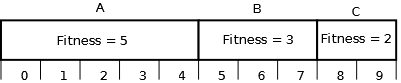
\includegraphics[scale=0.5]{../Stochastic.png}
	\end{figure}
	
\item Namespace: RoadNetworkFinder (See figures \ref{fig:RoadNetworkFinder} and \ref{fig:RoadNetworkFinderDependencies})
	\begin{itemize}
	\item RoadNetworkPopulator: An implementation of the IPopulator interface. This will randomly generate an initial population of RoadNetwork instances.
	\item RoadNetworkEvaluator: An implementation of the IEvaluator interface. This will calculate a fitness value for a RoadNetwork based on the total length of road and the distances from each town.
	\item RoadNetworkMutationOperator: An implementation of the IGeneticOperator interface. This will generate new individuals by randomly changing the best RoadNetworks in the current generation.
	\item RoadNetworkConjugationOperator: An implementation of the IGeneticOperator interface. This will choose pairs from the best individuals and randomly combine their parts to form new individuals.
	\item RoadNetworkOutputter: An implementation of the IOutputter interface. This will write the entire generation to a file.
	\item RoadNetwork: Represents a network of roads on a given map. This is used as the chromosome type for the RoadNetworkFinder plugins.
	\item Map: Represents the map supplied to the algorithm. Defines the extents of the map, start/end points of the road and locations of the towns.
	\item Vertex: Representes a vertex in a RoadNetwork.
	\item Edge: Represents an edge connecting two vertices in a RoadNetwork.
	\item Coordinates: A pair of integers giving an x-y location within a Map.
	\end{itemize}
	
\item Namespace: RoadNetworkFinderGUI (See figure \ref{fig:RoadNetworkFinderGUIDependencies})
	\begin{itemize}
	\item RoadNetworkFinderGUIMainWindow: Provides a graphical front-end to the GeneticEngine and PluginLoader classes for using the RoadNetwork plug-ins.
	\end{itemize}
	
\item Namespace: RoadNetworkVisualiser (See figure \ref{fig:RoadNetworkVisualiserDependencies})
	\begin{itemize}
	\item RoadNetworkVisualiserMainWindow: A GUI tool to load and view individuals from the files written by RoadNetworkOutputter.
	\end{itemize}

\end{itemize}

\paragraph{Class Diagrams}

\begin{figure}[ht!]
 \caption{Namespace: GeneticEngineCore}\label{fig:GeneticEngineCore}
 \centering
 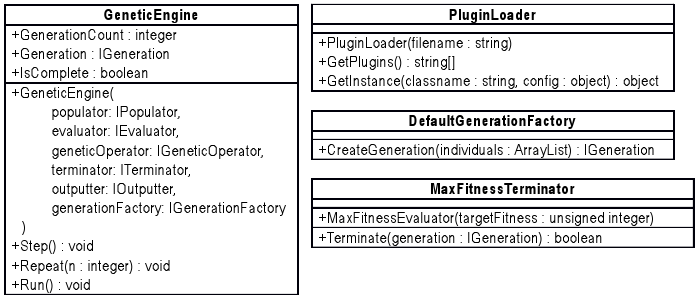
\includegraphics[width=\textwidth]{../GeneticEngineCoreDetail.png}
\end{figure}

\begin{figure}[ht!]
 \caption{Namespace: GeneticEnginePlugin}\label{fig:GeneticEnginePlugin}
 \centering
 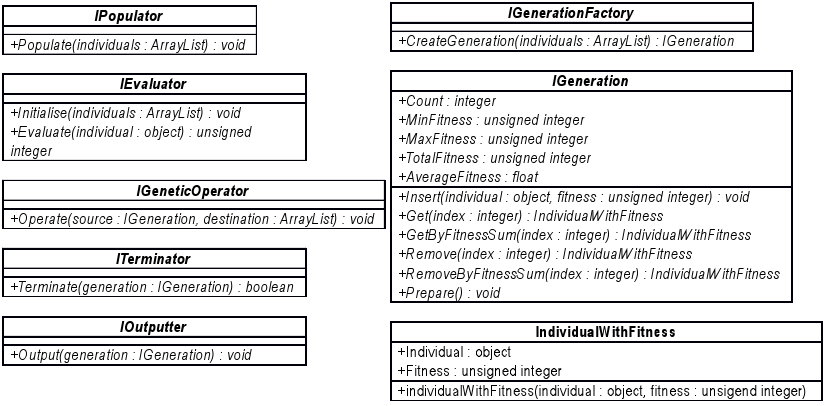
\includegraphics[width=\textwidth]{../GeneticEnginePluginDetail.png}
\end{figure}

\begin{figure}[ht!]
 \caption{Namespace: GeneticEngineSupport}\label{fig:GeneticEngineSupport}
 \centering
 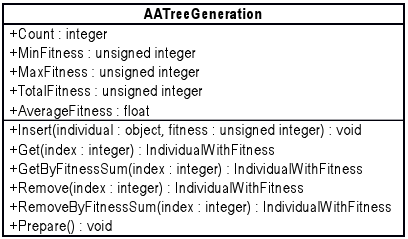
\includegraphics[width=0.5\textwidth]{../GeneticEngineSupportDetail.png}
\end{figure}

\begin{figure}[ht!]
 \caption{Namespace: RoadNetworkFinder}\label{fig:RoadNetworkFinder}
 \centering
 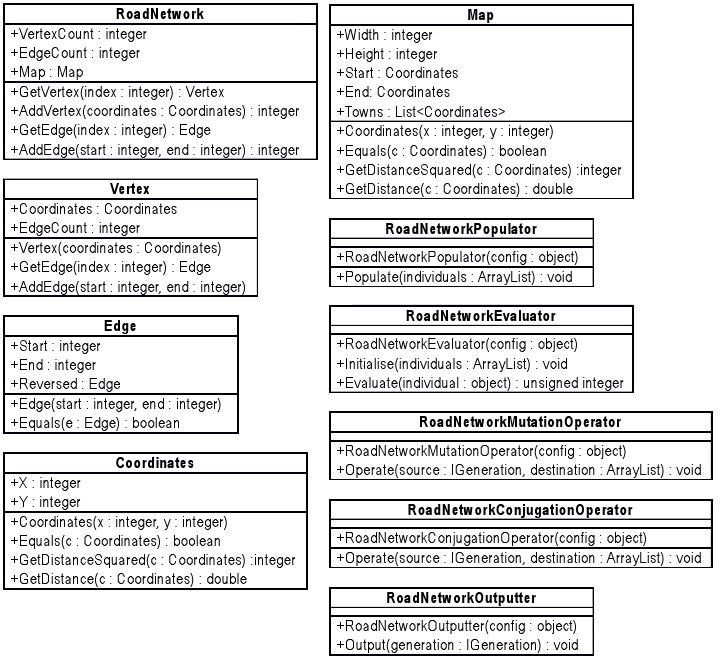
\includegraphics[width=\textwidth]{../RoadNetworkFinderDetail.png}
\end{figure}

\begin{figure}[ht!]
 \caption{GeneticEngineCore/Plugin/Support Dependencies}\label{fig:GeneticEngineDependencies}
 \centering
 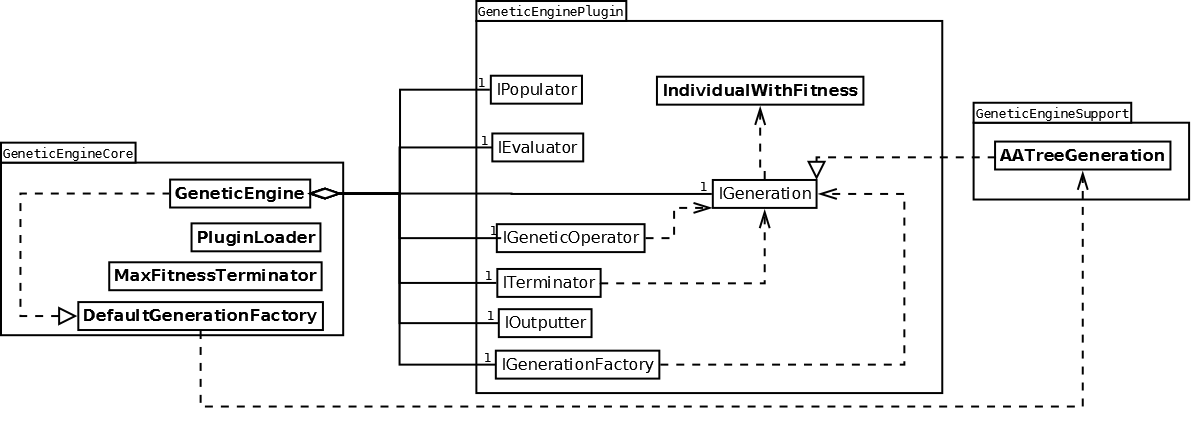
\includegraphics[width=\textwidth]{../GeneticEngineCorePluginSupport.png}
\end{figure}

\begin{figure}[ht!]
 \caption{RoadNetworkFinder Dependencies}
 \centering
 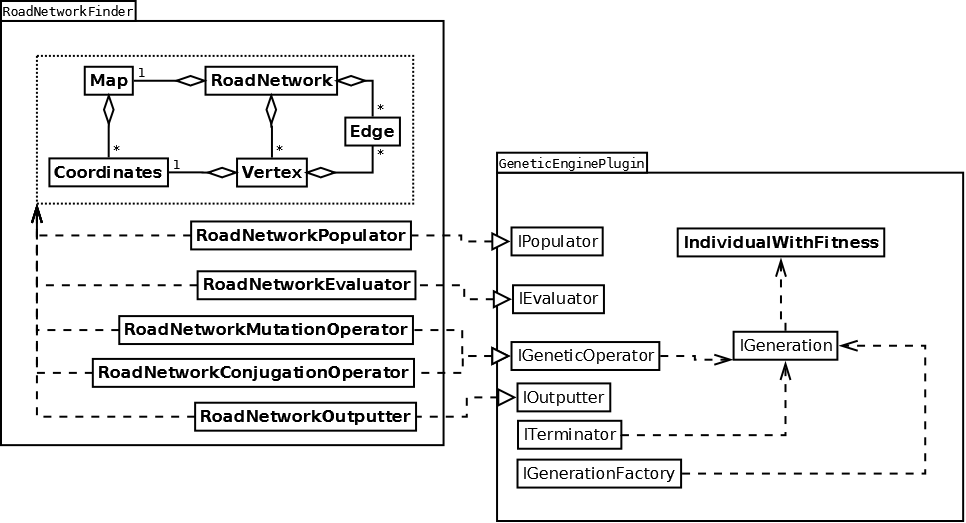
\includegraphics[width=0.7\textwidth]{../RoadNetworkFinder.png}\label{fig:RoadNetworkFinderDependencies}
\end{figure}

\begin{figure}[ht!]
 \caption{RoadNetworkFinderGUI Dependencies}
 \centering
 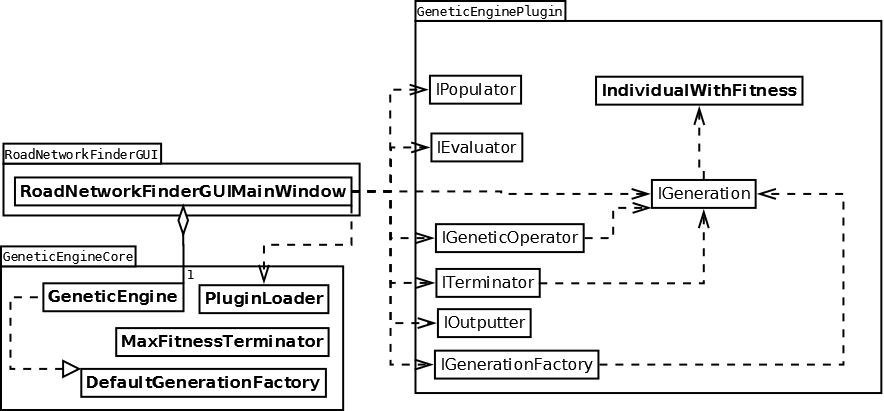
\includegraphics[width=0.7\textwidth]{../RoadNetworkFinderGUI.png}\label{fig:RoadNetworkFinderGUIDependencies}
\end{figure}

\begin{figure}[ht!]
 \caption{RoadNetworkVisualiser Dependencies}\label{fig:RoadNetworkVisualiserDependencies}
 \centering
 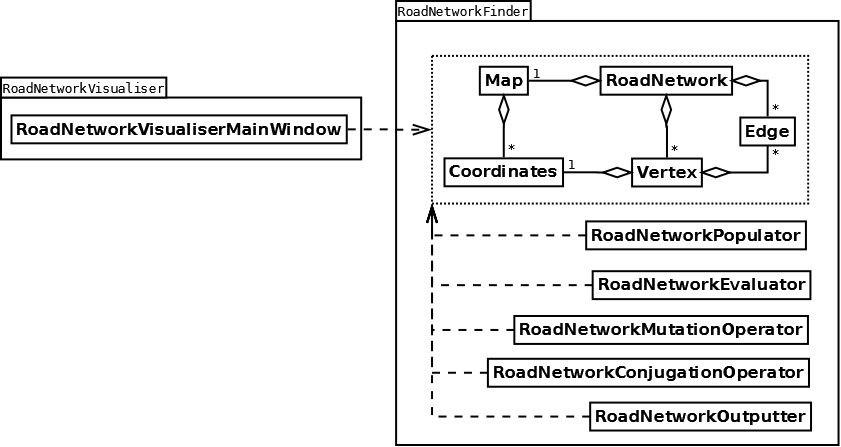
\includegraphics[width=0.7\textwidth]{../RoadNetworkVisualiser.png}
\end{figure}

\clearpage

% 3.5.4 - John
\subsubsection{Dynamic Models}

\begin{figure}[ht!]
 \caption{Sequence Diagram: Initialising and running the GeneticEngine from a client program.}\label{fig:Dynamic}
 \centering
 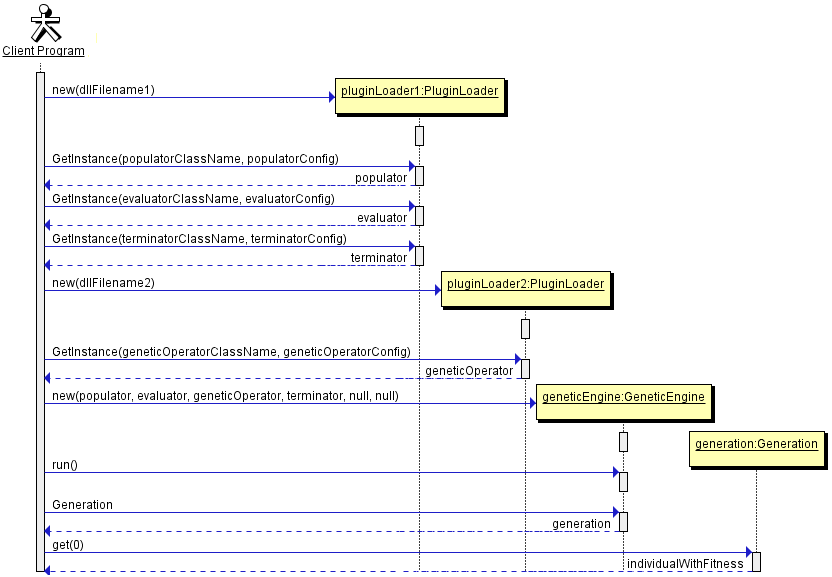
\includegraphics[width=\textwidth]{../Dynamic.png}
\end{figure}

In figure \ref{fig:Dynamic} the client program loads two dlls and gets instances of the plug-in classes from them. These classes are then used to instantiate the GeneticEngine class and run the algorithm. When it is complete the final generation is obtained and used to find the best individual.

\clearpage

% 3.5.5 - Brian
\subsubsection{User Interface - Navigational Paths and Screen Mockups}
\begin{figure}[ht!]
 \caption{Road Network Finder User Interface.}
 \centering
 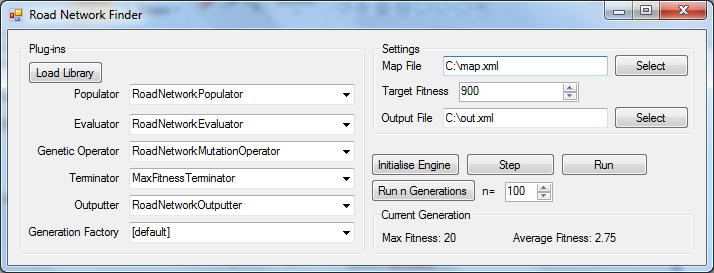
\includegraphics[width=0.75\textwidth]{../Finder.png}
\end{figure}

\begin{figure}[ht!]
 \caption{Road Network Visualiser User Interface}
 \centering
 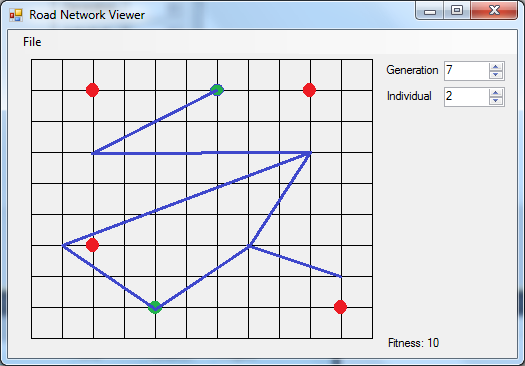
\includegraphics[width=0.75\textwidth]{../Visualiser.png}
\end{figure}

\clearpage

%\section{Glossary}
% TODO:

\end{document}
